\documentclass[../main/report.tex]{subfiles}
\begin{document}

\chapter{Physical Implementation}
\label{sec:pcb}

This chapter will describe the PCB layout, the main components and the design philosophy that went into solving the system requirements.
%\section{Layout Overview}
\section{Physical system structure}

\missingfigure{Physical overview}


\section{Design for Redundancy}

When designing a system the PCB is one of the harder things to debug.
If a wire inside the PCB is wrong, there is not munch that can be done, except buying a new PCB.
This becomes apparant when seeing most projects only have a working PCB on the 3rd of maybe even the 4th try.
Because of this, a strong philosophy has been used in the design for the PCB, as shown in figure \ref{fig:pcb_philosophy}.

To make sure the propability that a pcb will have a working design will be as high as possible, all aspects of the PCB has one or more backup plans.
All important wires and unused pins have been put onto headers, which can be rerouted manually.
That way each part can be connected to other parts of the board, or to other sources.
Because of this, the board is not optimized for size, but was rather made to optimize for highest possible chance of success.

Another part of this design is that each vital part of the PCB follows a modular design.
Each isolated part will work on its own, with the help of other components, if the rest of the board fails.
A PCB with a broken MCU, but with a functioning FPGA can be connected together and work as one system none the wiser.

\section{Main Components}

% Physical Overview
\section{Physical system structure}

\missingfigure{Physical overview}


% Design for Redundancy
\documentclass[../main/report.tex]{subfiles}
\begin{document}

\section{Design for Redundancy}

When designing a system the PCB is one of the harder things to debug.
If a wire inside the PCB is wrong, there is not munch that can be done, except buying a new PCB.
This becomes apparant when seeing most projects only have a working PCB on the 3rd of maybe even the 4th try. \todo{Citation needed}
Because of this, a strong philosophy of backup plans has been used in the design for the PCB, as shown in figure \ref{fig:pcb_philosophy}.

These backup plans are in place to make sure the board will work, even if some parts are broken.
All important wires and unused pins have been put onto headers, which can be rerouted manually.
That way, each component can be connected to other sources than that on the board alone.
Because of this, the board is not optimized for the smallest size possible, but was rather made to optimize for highest possible chance of success.

\end{document}


% Main Components
\documentclass[../main/report.tex]{subfiles}
\begin{document}

\section{Main Components}


\begin{description}

    \item[MCU (EFM32GG990F512-BGA112)] \hfill \\
    The EFM32 Giant Gecko Microcontroller from former Energy Micro, now Silicon Labs, was chosen as the microcontroller for this project.
    One aspect of the task at hand is energy efficiency and this microcontroller is particular efficient in that manner.
    This is a proven microcontroller with a lot of development boards available to us, so it seemed like a safe choice.

    \item[FPGA (XC6SLX45-2CSG324I)] \hfill \\
    The  FPGA of the Spartan-6 family from Xilinx was chosen as the FPGA.
    This particular FPGA has been used for different tasks on the university before, and the support systems are therefore available to us.
    The version was the one used on the PCB.
    A less powerful version of this one was available for testing on development boards in the lab.


    \item[SRAM] \hfill \\
    Yes yes, very good SRAM \todo{More here}

\end{description}

\end{document}


% Input
\documentclass[../main/report.tex]{subfiles}
\begin{document}

\section{Input}

The main method of communication between the microcontroller and a host PC is by USB.
The USB circuitry is designed with ESD protection in an effort to lessen the risk of frying the pcb. 
However, if the usb fails, a serial port(RS-232) has been implemented as a backup solution.
If this also fails, the wires from the serial port is put on headers, which can be used as GPIO pins.
If all else fails, the program to be run on the machine can be included when programming the MCU through the programming interface. 

\todo{Consider an image here}

\end{document}


% Output
\documentclass[../main/report.tex]{subfiles}
\begin{document}

\section{Output}
The main source of output from the FPGA is an HDMI connector.
This is a novel feature this year, as no previous group has tried to implement it before.

Because of this new challenge, a lot of backup schemes were put in place.
The HDMI connector is put on headers, in case the connector fails.
A separate VGA module is connected to the FPGA, in case the HDMI doesn't work and if this fails, a VGA module is also connected to the microcontroller.

\subsection{HDMI implementation}

The general HDMI specification consists of the Transition Minimized Differential Signaling(TMDS), and some additional wires for details regarding the transmitted signal \cite{hdmi-pinout}.
However, we were able to produce a video feed on a screen from an FPGA using only the TMDS wires by cutting up an HDMI cable and using only those wires.
Upon seeing that this was feasible, we decided to make the HDMI hardware with a TMDS connection only, going in to the FPGA. The resulting hardware was then an HDMI type-A receptacle footprint, the HDMI receptacle and a header between it and the FPGA.
The reason for adding the header was that this setup is equivalent to the aforementioned prototype version so that if the HDMI input wouldn't work we could connect the (header)terminated HDMI cable onto the header.

\todo{Consider an image here}

\end{document}


% Power
\documentclass[../main/report.tex]{subfiles}
\begin{document}

\section{Power}

The system is powered by a 5V mini usb.
The core design implementation is that this connection feeds electricity towards two voltage regulator circuits.
These, in turn power up the rest of the machine.
The usb connection has a backup solution in the form of a header through which the 5V line passes immediately after entering the pcb.
This is done so that the incoming electricity can easily be probed for voltage level and also so that in case the usb connection fails, an external power supply can be connected to the board.

\begin{figure}[H]
	\centering
	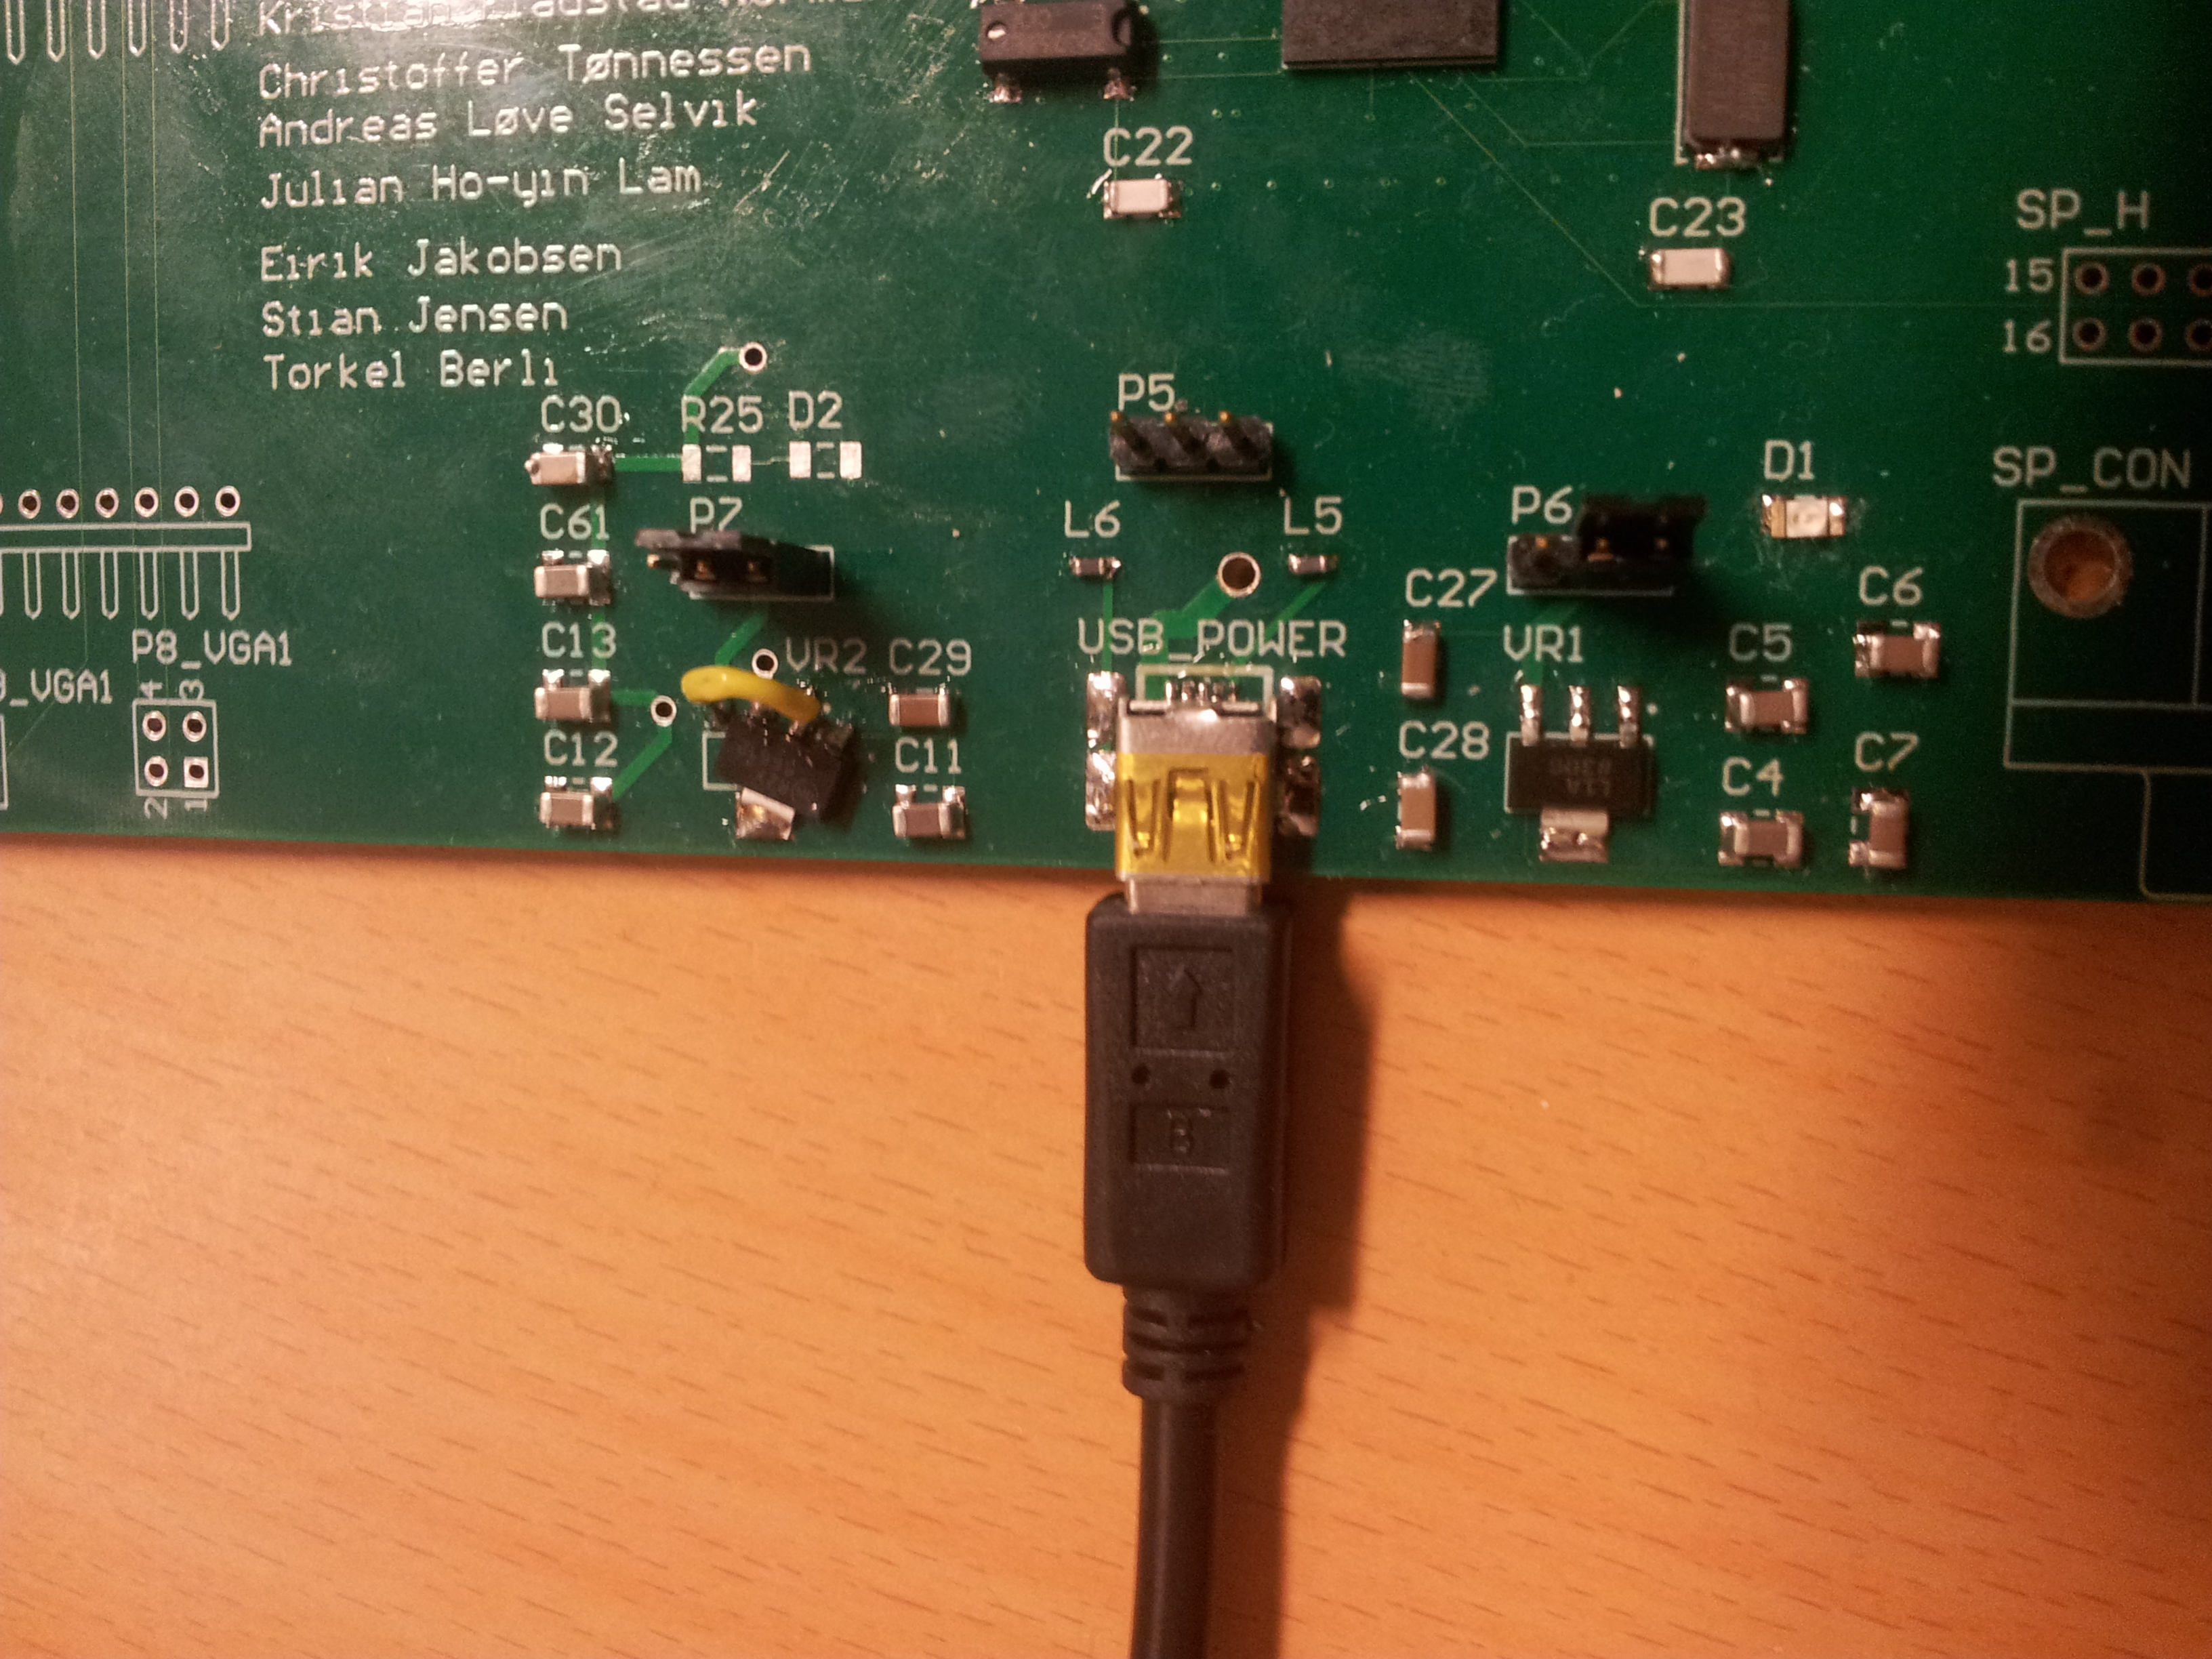
\includegraphics[width=0.65\textwidth]{../pcb/assets/power.jpg}
	\caption{Picture of physical power circuit}
	\label{fig: power picture}
\end{figure}
\todo{If the picture is to stay, should probably crop it a bit}

\end{document}


% Bus
\documentclass[../main/report.tex]{subfiles}
\begin{document}

\section{Bus}
The bus between MCU and FPGA is a standard EBI connection.
EBI stands for Extrenal Bus Interface, which is a parallel adress/data bus connecting multiple external components like SRAM, MCU, GPU etc etc.
The MCU have specific pins mapped for this protocol. /TODO{More Info about the EBI?}
Headers are placed in between the MCU and FPGA in case of failure on either side of the connection, as well as an easy way to check transmitted signals during debugging.

\end{document}


% Clocks
\documentclass[../main/report.tex]{subfiles}
\begin{document}

\section{Clocks}
Both the MCU and the FPGA need a external clock. The MCU need two crystals, a low frequency clock at 32.768kHz and a high frequencey clock at 48MHz. 
FPGA oscillator along with header on which an external oscillator resource can be connected by way of backup.
The microcontroller clocks on the other hand have a backup solution in that the microcontroller has internal RC-oscillators for use in case the crystals malfunction.

\end{document}


% HDMI?
\documentclass[../main/report.tex]{subfiles}
\begin{document}

\subsection{HDMI}

From a demo makers perspective, a GPU without a video output is commonly known as a space heater.
Demolicious uses HDMI for its video output, making it easy to connect to any recent video display.

HDMI is a streaming protocol; the receiver reads data from the cable at a fixed rate.
In Demolicious, the GPU has priority access to the memory.
This means that the video unit may not have access to the framebuffer (which lies in memory) when it's time to send a pixel.
To alleviate this issue, as much of the framebuffer as possible is prefetched into a buffer whenever memory is idle.
Should the buffer underflow, sending of late pixels must be abandoned.
Otherwise, pixels will not be synchronized with the position they should appear at on the screen.

Control signals assert where in the data stream a new frame of video starts and ends.
These allow the receiver to determine the resolution and refresh rate of the video.

The lowest resolution supported by HDMI is 640x480.
As this is larger than our framebuffers (64 x 64 pixels), a letterbox is added around the picture.
For debugging purposes, the letterbox consists of a low-contrast checker pattern.

To actually send the data over HDMI, control signals and pixel data are split into three channels.
They are then encoded using a scheme known as TMDS.
The purpose of TMDS is to minimize the effect of noise over the physical connection.

TMDS uses 10 bits to encode either an 8-bit color value when sending a image, or control values when not.
Demolicious uses a 16-bit word size, so colors are represented with 5 bits for red, 6 for green and 5 for blue.
These are resized to 8-bit values using a scheme that allows for both complete black and white colors.
Each channel is then serialized before being output together with a clock using differential-signaling.

Finally, to avoid a visual artifact known as \emph{screen tearing}, a technique known as \emph{V-sync} with \emph{double buffering} is used.
These techniques ensure that only complete frames of video are output, increasing visual fidelity.

\end{document}


\section{Footprints}
Predominantly SMDs(surface mounted device) large enough for humans to solder(with a couple of exceptions)

\subfile{../pcb/hdmi.tex}

\todo{...Uncertain ie om at vi endra litt på en del footprints, men pga hvordan fysiske komponenter funker,}

\subsubsection{Prebundled}

\subsubsection{Handmade}
Some footprints we had to make ourselves.
This was done inside Altium.
The specification for the footprints was found in the datasheets of the component in question.

When making the handmade footprints some other thoughts were taken into account.

\begin{itemize}
    \item We need to solder these components
    \item The connection on the components is physical, as long as it leads current, it will work.
    \item Some datasheets didn't match the component exactly, but was for a sister component
\end{itemize}

With this in mind we made footprints which was slightly bigger than it needed to.

\begin{verbatim}
Needed:                 Actual:
--------------          --------------
|            |          |            |
|--|      |--|       |--|--|      |--|--|
|  |      |  |       |  |  |      |  |  |
|..|      |--|       |--|..|      |--|--|
|            |          |            |
--------------          --------------
\end{verbatim}
\end{document}
